%==================================================================%
% Author : Pando Muñoz, Manuel                                     %
%          Sánchez Barreiro, Pablo                                 %
% Version: 1.0, 02/03/2011                                         %
%                                                                  %
% Memoria del Proyecto Fin de Carrera                              %
% Archivo raíz para el capítulo de iteración                       %
%==================================================================%

\chapterheader{Segunda iteración}{Descripción de una iteración}
\label{chap:iteracion}

\chaptertoc

En el siguiente capítulo se describe lo realizado en la segunda iteración de construcción.
Se parte de lo obtenido en las iteraciones previas, que es, la descripción del sistema, la arquitectura del mismo y los diagramas de secuencia y estados, todo esto expuestos a lo largo de los capítulos \ref{chap:planificacion} \ref{chap:arquitectura}.
En cuanto al estado de la aplicación, en la primera iteración de construcción se ha desarrollado un sistema distribuido, en el que desde la aplicación del alumno se puede conectar con la aplicación del profesor y transmitir ficheros.
El objetivo de esta iteración es que el profesor pueda establecer el inicio y de la prueba, poder prefijar una hora de finalización de la misma y que la aplicación del alumno sea capaz de denegar el acceso a la red mientras dure la prueba. %
En las siguientes secciones se describen los incrementos realizados dentro de esta iteración.

%contar el desarrollo del daemon
%contar como utilizo iptables
%Secciones: Inicio de prueba, Examen temporizado, Denegar acceso red

\section{Inicio de la prueba}
\label{sec:iteracion:iniPrueba}

En esta sección se comenta cómo se consigue que el profesor pueda notificar a los alumnos el inicio de la prueba.
Como ya hemos comentado, partimos de la iteración anterior en la cual los alumnos eran capaces de conectar a la aplicación del profesor. En la aplicación del alumno, cuando se crea una conexión, se inicia a su vez un hilo de ejecución que se mantiene a la espera de recibir distintas órdenes provenientes del computador del profesor. De este modo se hace muy simple mantener desde la aplicación del profesor una lista de las conexiones abiertas con cada alumno y, al presionar el botón de iniciar la prueba, recorrer esa lista enviando la orden por cada conexión.

Cuando cada una de las aplicaciones del alumno recibe esa orden, actúa en consecuencia.

\section{Examen temporizado}
\label{sec:iteracion:examenTemporizado}

El profesor puede establecer una hora límite, llegada la cual, la prueba terminará automáticamente. Cuando el profesor define este límite en su aplicación y decide comenzar la prueba se envía también si hay una hora de fin y, en caso afirmativo, cual es. De este modo la aplicación del alumno puede mostrar una cuanta atrás con los minutos restantes para la finalización, para facilitar la referencia temporal. Se puede ver el resultado en la siguiente imagen.

\begin{figure}[!htb]
    \centering
    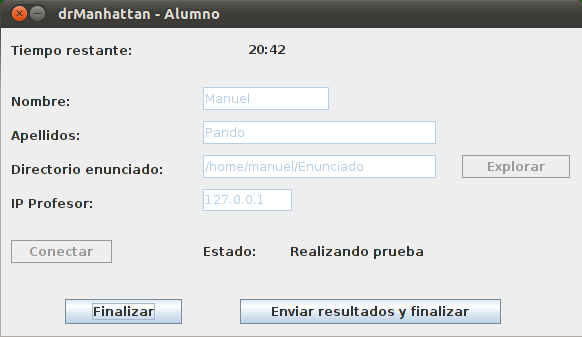
\includegraphics[width=.75\linewidth]{iteracion/tiempoRestante}
    \caption{Aspecto de la GUI del alumno con una prueba temporizada.}
    \label{fig:iteracion:tiempoRestante}
\end{figure}


\section{Denegar acceso a red}
\label{sec:iteracion:denegarRed}

Cómo ya hemos visto en las secciones anteriores, una vez que la aplicación del alumno recibe la orden de comenzar la prueba, se ha de denegar el acceso a la red. Para ello se utiliza iptables, por medio de un demonio.

El demonio creado es muy simple, se ejecuta en segundo plano esperando a que la aplicación del alumno conecte, y en función de lo requerido en ese momento, permitir o no el acceso a la red interactuando con iptables. Este demonio se inicia en tiempo de arranque y con los permisos necesarios para poder usar el cortafuegos.


\section{Pruebas}
\todo{tema seguridad de que no se puede acceder a red}
